\section{Laplace Transform}

Laplace transform of a function $F(t)$ denoted by $\mathcal{L}\{F(t)\}$. The Laplace operator $\mathcal{L}$ is linear, so

\begin{equation*}
    \mathcal{L}\{c_1f_1(t)+c_2f_2(t)\}=c_1\mathcal{L}\{f_1(t)\}+c_2\mathcal{L}\{f_2(t)\}
\end{equation*}

Defined as

\begin{equation*}
    \mathcal{L}\{F(t)\}=\int_0^\infty e^{-st}F(t)dt
\end{equation*}

Integral is a function of parameter $s$, say $f(s)$ such that $\mathcal{L}\{F(t)\}=f(s)$.
Improper integral will always converge, and can be written as a limit definition:

\begin{equation*}
    \int_0^\infty e^{-st}F(t)dt=\lim_{A\to \infty}\int_0^Ae^{-st}F(t)dt
\end{equation*}

We can derive some general forms based on this idea.

\subsection{Laplace transform definitions}

\begin{definition}($\mathcal{L}\{e^{kt}\}$)\\
    Finding $\mathcal{L}\{e^{kt}\}$ for $s>k$ (condition for convergence), we see that 

    \begin{equation*}
        \mathcal{L}\{e^{kt}\}=\lim_{A\to\infty} \int_0^A e^{-st}e^{kt}dt=\lim_{A\to\infty}\frac{1}{k-s}e^{(k-s)t}\mbox{$\mathcal{L}$\Large$\mid$}_0^A=\frac{1}{s-k}
    \end{equation*}
\end{definition}

\begin{definition}($\mathcal{L}\{\sin kt\}$)\\
    Evaluating the integral:
    \begin{align*}
        \int e^{-st}\sin kt&=-\frac{1}{k}e^{-st}\cos kt-\int se^{-st}\frac{1}{k}\cos kt \;dt\\
        &=-\frac{1}{k}e^{-st}\cos kt-\frac{s}{k}\int e^{-st}\cos kt \;dt\\
        &=-\frac{1}{k}e^{-st}\cos kt-\frac{s}{k}\left( \frac{1}{k}e^{-st}\sin kt-\int -\frac{s}{k}e^{-st}\sin kt\;dt \right)\\
        &=-\frac{1}{k}e^{-st}\cos kt-\frac{s}{k}\left(\frac{1}{k}e^{-st}\sin kt + \int \frac{s}{k}e^{-st}\sin kt\;dt\right)\\
        (1+\frac{s^2}{k^2})\int e^{-st}\sin kt&=-\frac{1}{k}e^{-st}\cos kt-\frac{s}{k^2}e^{-st}\sin kt\\
        \frac{k^2+s^2}{k^2}\int e^{-st}\sin kt&=\frac{1}{k}e^{-st}\cos kt-\frac{s}{k^2}e^{-st}\sin kt\\
        \int e^{-st}\sin kt&=-\frac{ke^{-st}\cos kt}{k^2+s^2}-\frac{se^{-st}\sin kt}{k^2+s^2}\\
        &=-\frac{e^{-st}}{k^2+s^2}\left(k\cos kt-s\sin kt\right)
    \end{align*}

    So evaluating the improper integral,
    
    \begin{align*}
        \left[-\frac{e^{-st}}{k^2+s^2}\left(k\cos kt-s\sin kt\right)\right]_0^\infty&=0+\frac{1(k-0)}{s^2+k^2}\\
        &=\frac{k}{s^2+k^2}
    \end{align*}

    It can be similarly obtained that $\mathcal{L}\{\cos kt\}=\frac{s}{s^2+k^2}$ (for $s>0$ in both cases).
\end{definition}

\begin{definition}($\mathcal{L}\{t\}$)
    \begin{align*}
        \mathcal{L}\{t\}&=\int_0^\infty e^{-st}tdt\\
        &=\lim_{A\to\infty}\int_0^A\underbrace{e^{-st}}_{dv}\underbrace{t}_{u}dt\\
        &=\lim_{A\to\infty}\left[ -\frac{1}{s}e^{-st}t\bigg\rvert_0^A-\int_0^A -\frac{1}{s}e^{-st}dt \right]\\
        &=\lim_{A\to\infty}\left[-\frac{1}{s}e^{-st}t-\frac{1}{s^2}e^{-st}\right]_0^A\\
        &=-\left[-\frac{1}{s^2}\right]=\frac{1}{s^2}
    \end{align*}
\end{definition}

\begin{definition}($\mathcal{L}\{\sin^2 at\}$)
    \begin{align*}
        \mathcal{L}\{\sin^2 at\}&=\mathcal{L}\{\frac{1}{2}(1-\cos 2at)\}=\frac{1}{2}\mathcal{L}\{1\}-\frac{1}{2}\mathcal{L}\{\cos 2at\}
    \end{align*}
\end{definition}

\begin{definition}(Transforms of Derivatives)
    If $F(t)$ is continuous for $t\geq 0$ and of exponential order as $t\to \infty$, then we can simplify

    \begin{align*}
        \mathcal{L}\{F'(t)\}&=\int_0^\infty e^{-st}F'(t)\;dt\\
        &=\left[e^{-st}F(t)\right]_0^\infty+s\int_0^\infty e^{-st}F(t)\;dt\\
        &=-F(0)+s\mathcal{L}\{F(t)\}
    \end{align*}

    Useful fact that can be resubstituted for \[\mathcal{L}\{F''(t)\}=-F'(0)+s\mathcal{L}\{F'(t)\}=-F'(0)-sF(0)+s^2\mathcal{L}\{F(t)\}.\]

    General form:

    \begin{equation*}
        \mathcal{L}\{f^n(t)\}=s^n\mathcal{L}\{f(t)\}-s^{n-1}f(0)-s^{n-2}f'(0)-s^{n-3}f''(0)-\ldots-f^{n-1}(0)
    \end{equation*}
\end{definition}

\begin{definition}(Translation property)
    \begin{equation*}
        \mathcal{L}\{e^{at}f(t)\}=\int_0^\infty e^{-st}e^{at}f(t)dt=\int_0^\infty e^{-(s-a)t}f(t)dt=F(s-a)
    \end{equation*}
\end{definition}

\begin{definition}($\mathcal{L}\{t^nf(t)\}$)
    \begin{align*}
        \mathcal{L}\{t^nf(t)\}=(-1)^n\frac{d^n}{ds^n}\mathcal{L}\{f(t)\}
    \end{align*}    
\end{definition}

\subsection{Solving DEs}

Approach to solving DEs involves applying Laplace to both sides of some DE

\begin{equation*}
    F(y)=f(t)
\end{equation*}

and isolating $Y(s)=\mathcal{L}\{y(t)\}$ using the derivative transform. Then, use
the inverse Laplace transform and linearity property to find $y(t)$ from $Y(s)$.

\subsection{Step Function}

\begin{figure}[H]
    \centering
    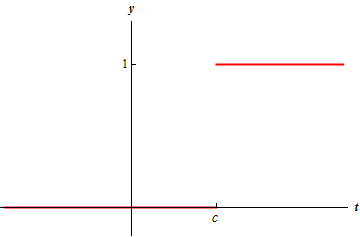
\includegraphics[scale=.5]{figures/unitstep.png}
    \caption{Unit step function}
\end{figure}

The unit step function centered at $a$ is defined as

$$
u_a(t)=u(t-a)=\begin{cases}
    0,t<a\\
    1,t\leq a
\end{cases}
$$

Can define rectangular step function with pulse width $b-a$ where $b>a$:

\begin{equation*}
    r(t)=u(t-a)-u(t-b)
\end{equation*}

Calculating the Laplace transform is simple:

\begin{align*}
    \mathcal{L}\{u_a(t)\}&=\int_0^a e^{-st}(0)dt + \int_a^\infty e^{-st}dt\\
    &=-\frac{e^{-st}}{s}\bigg\vert_a^\infty=\frac{e^{-sa}}{s}
\end{align*}

\begin{definition}(Step Function Translation)

    Let there be some arbitrary curve $f(t)$ defined for all $t$ and the step function $u(t-a)$.
    The new function $u(t-a)f(t-a)$ gives the step function with shape $f(t-a)$ for $t>a$. Applying the Laplace transform, we get

    \begin{align*}
        \mathcal{L}\{u(t-a)f(t-a)\}&=\int_0^\infty e^{-st}u(t-a)f(t-a)dt\\
        &=\int_0^a e^{-st}(0)dt+\int_a^\infty e^{-st}f(t-a)dt\\
    \end{align*}

    Let $x=t-a\implies t=x+a$. Further note that when differentiating, $dx=dt$, making this substitution useful.

    \begin{align*}
        \int_0^a e^{-st}(0)dt+\int_a^\infty e^{-st}f(t-a)dt&=\int_a^\infty e^{-s(x+a)}f(x)dt\\
        &=e^{-sa}\int_a^\infty e^{-sx}f(x)dx\\
        &=e^{-sa}\mathcal{L}\{f(t)\}
    \end{align*}
\end{definition}

\subsection{Periodic Functions}

\begin{definition} (Periodic Laplace Transform)
    If $f(t)$ is periodic, then $f(t-P)=f(t)$ (for $t\geq P$) and
    \begin{equation}
        \mathcal{L}\{f(t)\} = \displaystyle\frac{\int_0^Pe^{-st}f(t)dt}{1-e^{-Ps}}
    \end{equation}
\end{definition}

\begin{proof}
    We can write the transform as two integrals,
    \begin{align}
        F(s)&=\int_0^P e^{-st}f(t)dt + \int_P^\infty e^{-st}f(t)dt\\
        &= \int_0^P e^{-st}f(t)dt + \int_P^\infty e^{-st}f(t+P)dt\label{split}
    \end{align}

    Note that $\tau = t-P\implies t=\tau +P$ so $dt = d\tau$.
    \begin{align}
        \int_P^\infty e^{-st}f(t+P)dt &= \int_{2P}^\infty e^{-s(\tau + P)}f(\tau)d\tau\\
        &= e^{-sP}\int_{0}^\infty e^{-s\tau}f(\tau)d\tau\\
        &= e^{-sP}F(s)
    \end{align}
    Substituting into \ref{split}, we get
    \begin{equation}
        F(s)=\int_0^P e^{-st}f(t)dt + e^{-st}F(s)\implies (1-e^{-sP})F(s)=\int_0^P e^{-st}f(t)dt
    \end{equation}
\end{proof}

\subsection{Convolution Operation}

\begin{definition} (Convolution Theorem)
    \begin{equation}
        f * g = \int_0^t f(r) g(t-r)dr=g * f
    \end{equation}
    Applying the Laplace operator,
    \begin{equation}
        \mathcal{L}\{f*g\}=\mathcal{L}\{f(t)\}\mathcal{L}\{g(t)\}=F(s)G(s)
    \end{equation}
    A more useful property is of the inverse,
    \begin{equation}
        f*g=\mathcal{L}^{-1}\{F(s)G(s)\}
    \end{equation}
\end{definition}

\begin{example}
    Finding the the inverse transform, we can apply the Laplace convolution definition,
    \begin{align*}
        \mathcal{L}^{-1}\{\frac{a}{s^2(a^2+s^2)}\}&=\int_0^t (t-u)\sin au\,du\\
        &=t\int_0^t \sin au\, du -\int_0^t u\sin au\, du\\
        &=-t(\cos at - 1)-\left(-u\cos au\bigg\vert_0^t+\int_0^t \cos au\,du\right)\\
        &=t(1-\cos at)+t\cos at+\sin at
    \end{align*}
\end{example}

\subsection{Integral Transform}